% id: 34-01
% book: 베이직쎈 확률과 통계 · 02 중복조합과 이항정리
% section: 실전 감각 UP
% figure: crop:fig-34-01.jpg
% answer: 
% answer_source: 
% variant_level: 0 (원본 전사)
% 이 파일은 build.mjs 가 items.json 에서 만든다. 고칠 때는 items.json 을 고친다.
\smash{\raisebox{1.5mm}{\dmkichul{베이직쎈 확률과 통계 34쪽 01번}}}
\noindent\begin{minipage}[t]{0.58\linewidth}\vspace{0pt}\raggedright 오른쪽 그림은 어느 음료 가게의 메뉴판이다. 선희가 이 가게에서 메뉴판에 있는 음료 중 7개의 음료를 주문하는 경우의 수는?\end{minipage}\hfill\begin{minipage}[t]{0.4\linewidth}\vspace{0pt}\centering 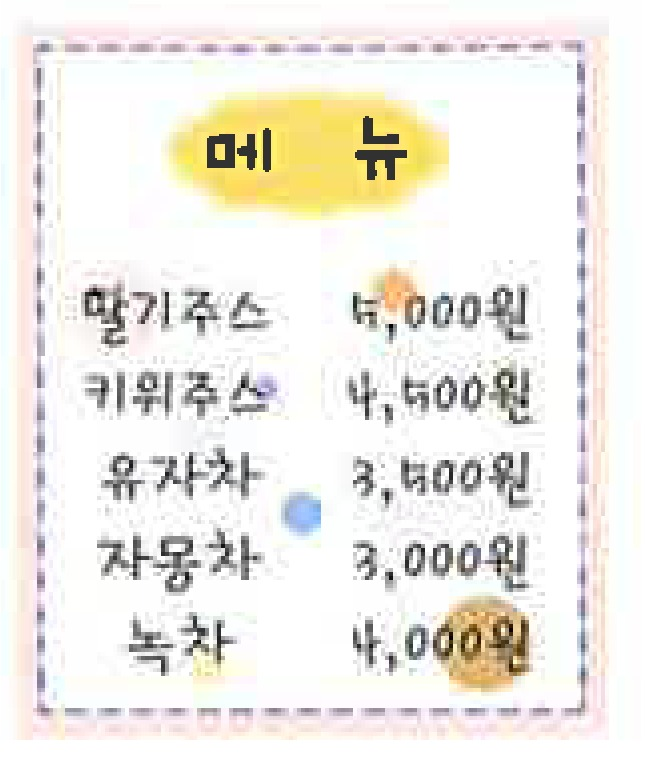
\includegraphics[width=0.92\linewidth]{figures/fig-34-01.jpg}\end{minipage}\par
\dmchoicesauto{}{$170$}{$210$}{$250$}{$290$}{$330$}
